\begin{figure}
    \footnotesize
\noindent
\tcbsetforeverylayer{autoparskip}
\tcbset{enhanced, nobeforeafter, width=1\linewidth}
\begin{tcolorbox}[sidebyside,arc=0.5mm, 
    colback=MidnightBlue!10!white, 
    coltext=MidnightBlue!90!black,  
    colframe=MidnightBlue!90!black,
    colbacktitle=MidnightBlue!80,
    leftrule=0mm,
    rightrule=0mm, 
    toprule=0mm, 
    bottomrule=0mm,
    box align=top,
    title={\begin{panel}Transitional distribution \label{pan:transitional}\end{panel}}]

The \gls{ehrgan} generator is trained to decode a random vector $z$ mixed with the latent space representation of a real patient $h$ to produce a synthetic sample $\tilde{x}$ \cite{Che_2017}. A standard autoencoder (left) is trained to encode a real patient $x$ to and from a latent representation $h$, minimizing the reconstruction error with $\Bar{x}$. The decoder portion (left) is then trained to produce realistic synthetic samples $\tilde{x}$ from a combination of the random latent vector $z$ and the latent space encoding of a real patient $x$. The generator thus learns a transition distribution $p(\tilde{x}|x)$ with $x \thicksim p_{data}(x)$. The amount of contribution of the real sample is controlled by a random mask according to $\tilde{h} =m * z + (1 - m) \cdot h$. This method inspired from Variational Contrastive Divergeance prevents mode collapse by design and  learns an information rich transition distribution $p(\tilde{x}|x)$ around real samples $x$.
\tcblower
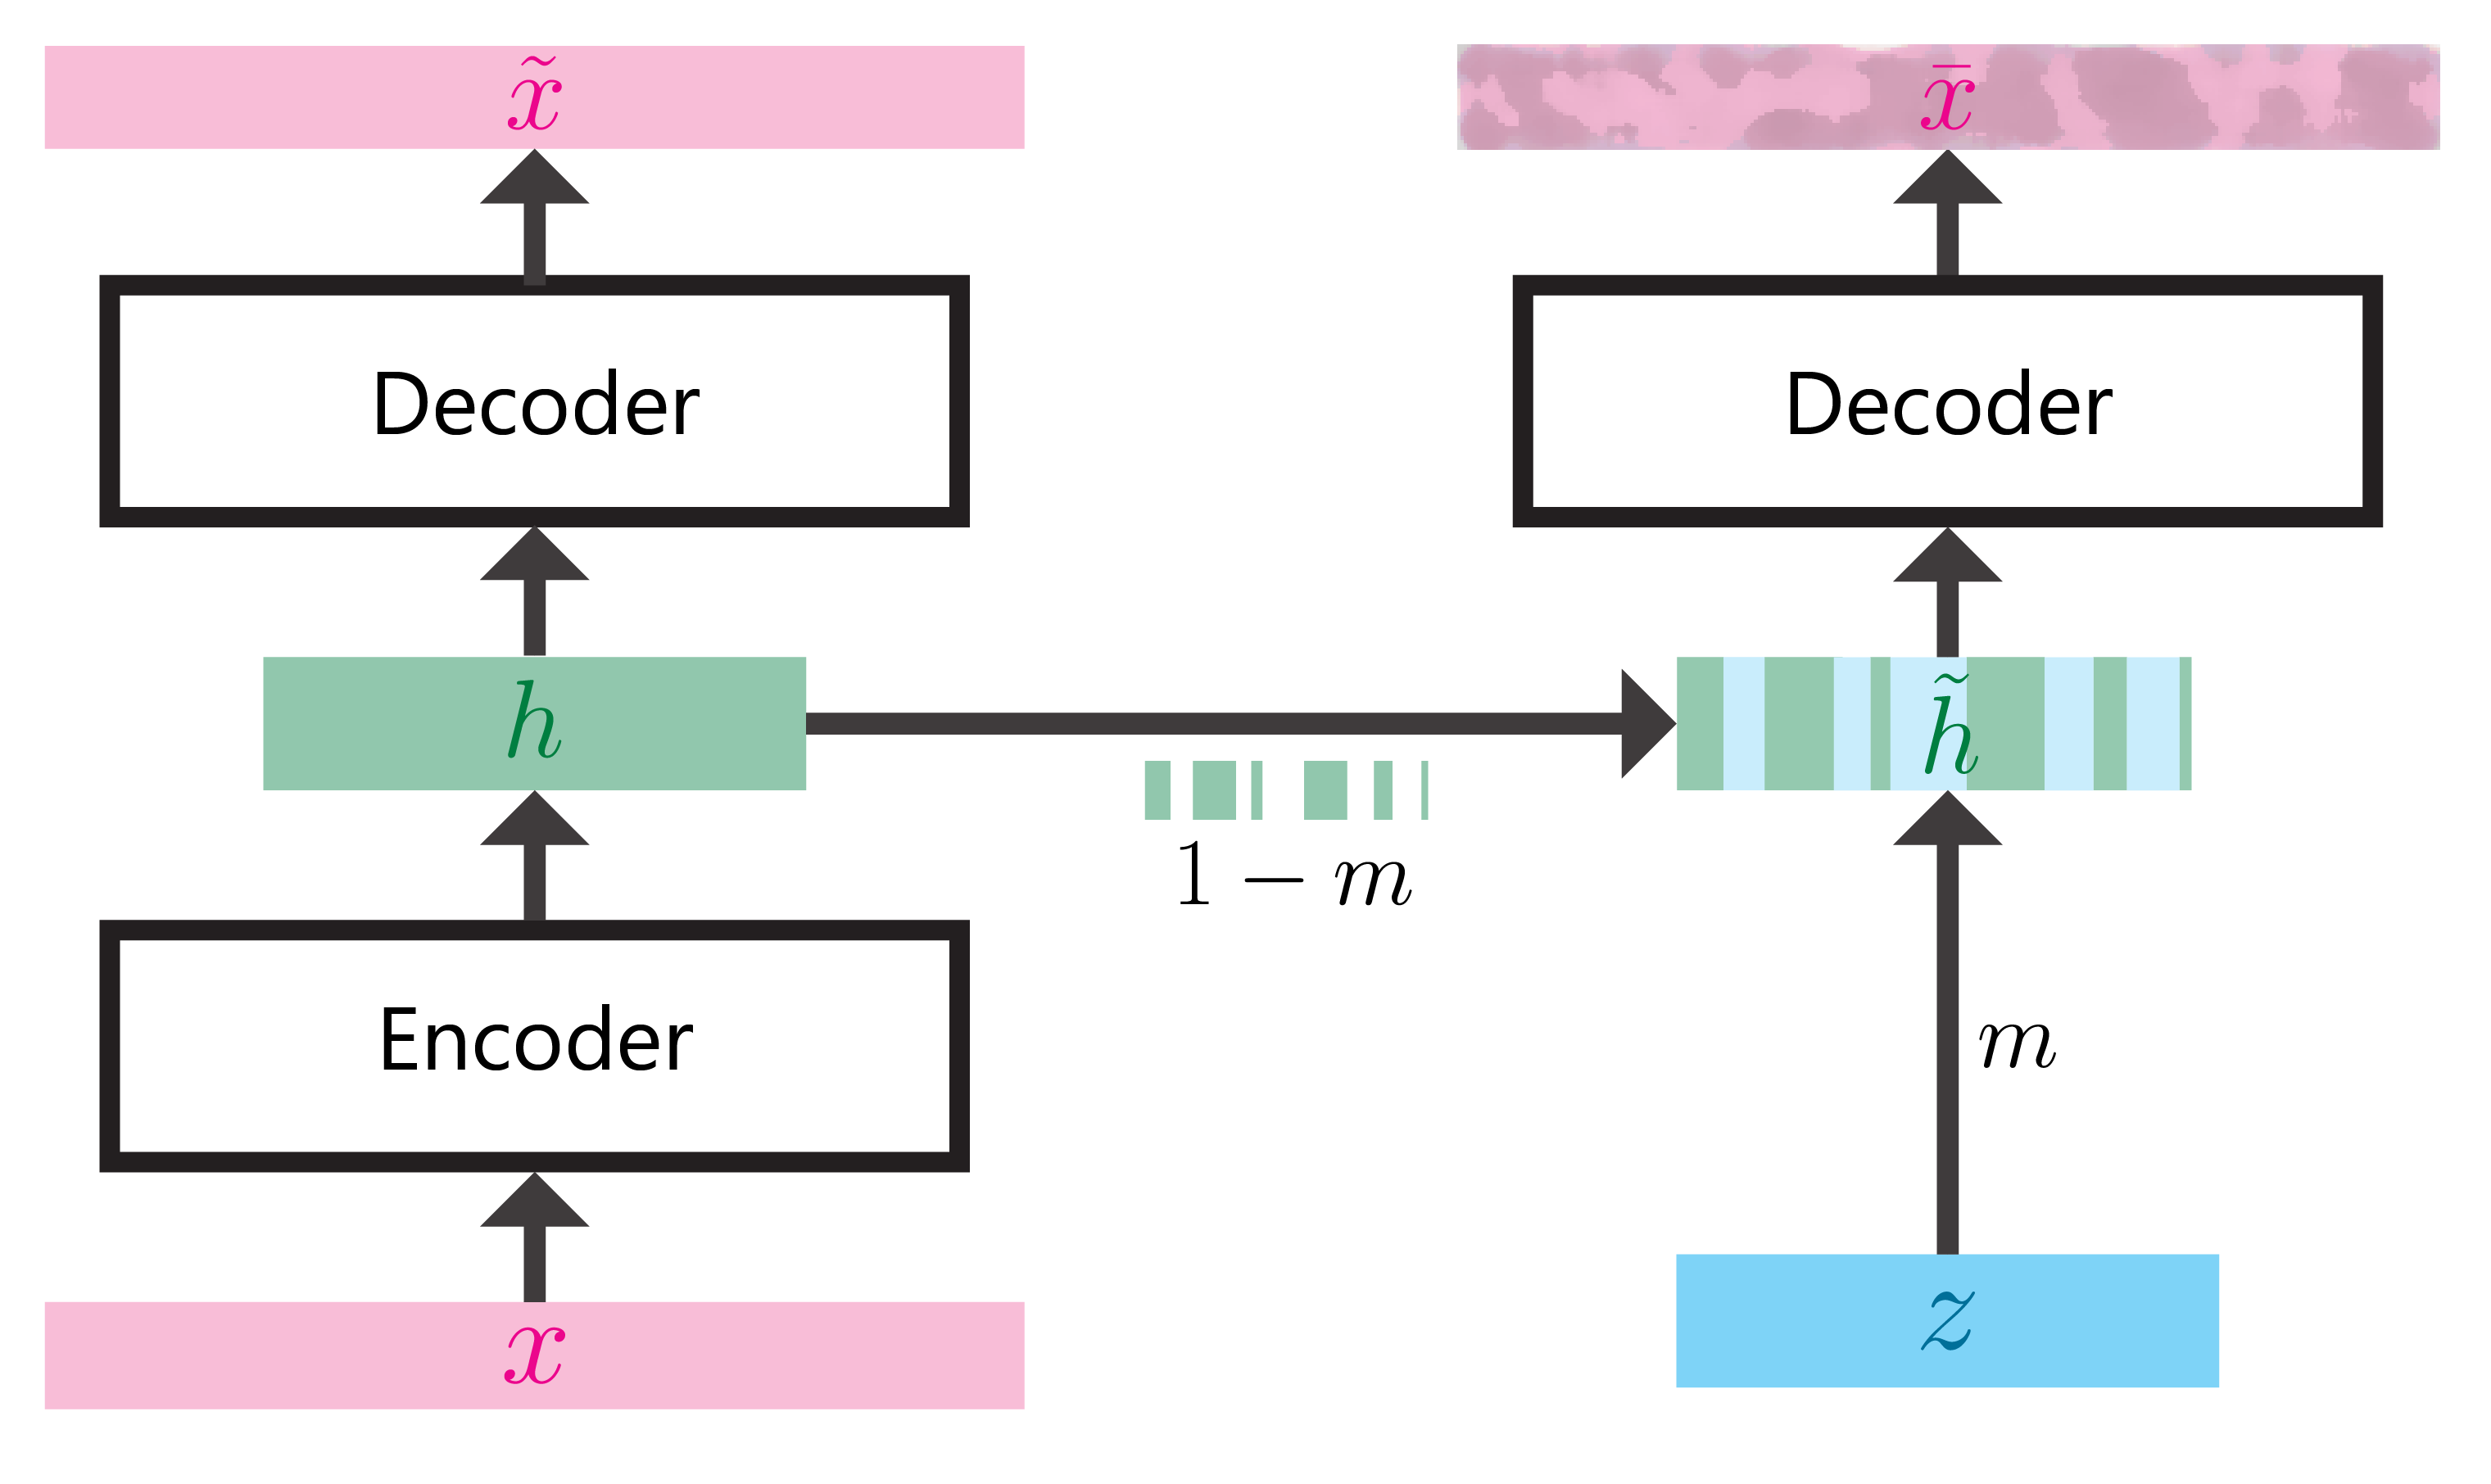
\includegraphics[width=1\columnwidth]{assets/transitional}
\end{tcolorbox}
\normalsize
\end{figure}